\section{Proton-Proton Collisions at the LHC}
\subsection{An Introduction to Particle Accelerators and Detectors}\label{subsec:Detector}
With a circumference of 27 km, the \acf{LHC} \emph{particle accelerator} is the largest piece of scientific 
equipment ever built. It consists of two separate large tubes aligned with powerful magnets. An electromagnetic field is
applied to accelerate bunches\footnote{Packets of around $10^{11}$ protons each.} of charged hadrons (specifically protons) and lead,
and the magnets are used to bend and focus the bunches. One set of bunches are accelerated in one of the tubes, 
and another set is accelerated in the other direction inside the other tube. The bunches are accelerated to relativistic speeds.
(v=0.99999991c) before they collide at a rate of once every 25 nanosecond. The energy released from 
the collisions enable the creations of new particles.
\\
To measure the outcome of the collisions, we use \emph{particle detectors}. In this thesis I will be using data collected by the 
\acs{ATLAS} (\acl{ATLAS}) detector. The \ac{ATLAS}-detector is the largest general-purpose detector at the \ac{LHC}
and took first data from particle collisions in 2009. The detector consists of several layered cylinders and end-caps 
around the point of collision. In figure \ref{fig:detector}, taken from the \ac{ATLAS} collaboration \cite{PDetector} the cross-section 
of the detector along with the paths of different particles is visualized. The inside of a detector can be summarized 
in the following points, listed from innermost to outermost layer:
\begin{itemize}
    \item \emph{Inner Detector}: The inner detector consists of three layers, Pixel detector, Semi-Conductor Tracker 
          and Transition Radiation Tracker. Its purpose is to measure \ac{EM} interactions between the particles 
          produced in the collision and the material in the layers. The measurements are made at discrete points and can be 
          used to infer the trajectories of the particles. A magnetic field is applied to the inner detector
          to bend the paths of the particles, enabling the measurement of the momentum and charge.  
    \item \emph{Calorimeters}: The \ac{ATLAS} detector has two types of calorimeters, the \emph{Electromagnetic calorimeter} and the 
           \emph{Hadronic calorimeter}. The \ac{EM} calorimeter is the first layer of the two and measures the energy of 
           photons and electrons interacting electromagnetically. The hadronic calorimeter is designed to measure the energy of 
           hadrons (i.e. protons, neutrons, mesons etc.).
    \item \emph{Muon Spectrometer}: Contrary to electrons, photons and hadrons, the muons do not stop in the calorimeters.
            The muon spectrometer measures their trajectories in the outer part of the detector allowing the extrapolation of
            the path from the inner detector to muon spectrometer. Similarly to the inner detector, the muon spectrometer 
            is surrounded by a magnetic field to deflect the path of the particles which allows it to measure momentum and charge. 
\end{itemize}
\begin{figure}
    \centering
    \makebox[0.75\linewidth][c]{%
    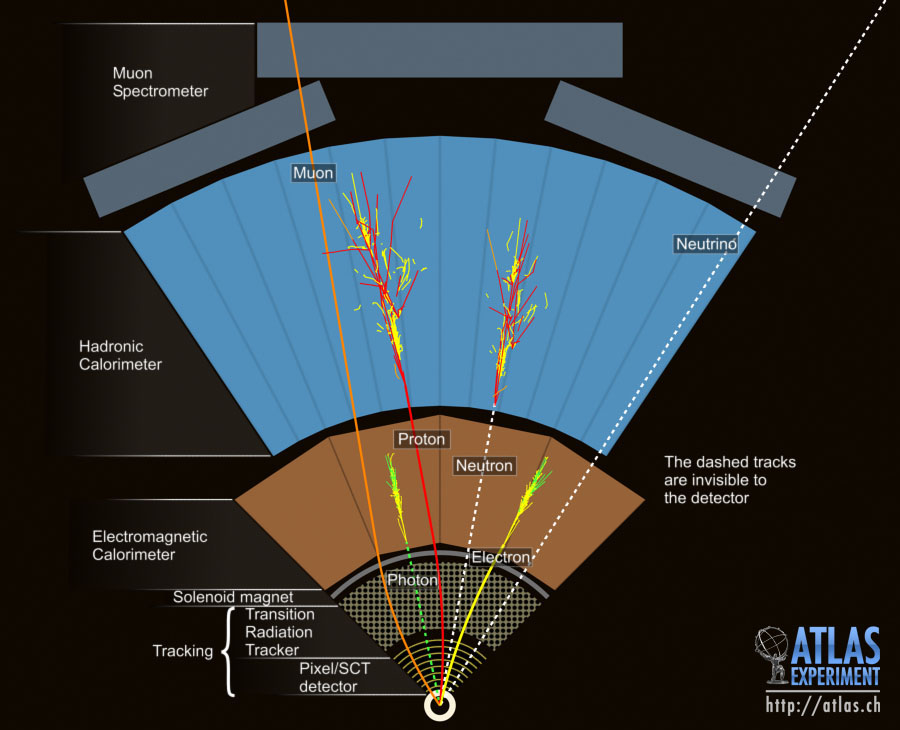
\includegraphics[width=0.75\textwidth]{Figures/Illustrations/detector.jpeg}
    }
    \caption[Event Cross Section in a computer generated image of the
    \acs{ATLAS} detector.]{Event Cross-Section in a computer generated image of the
    ATLAS detector \cite{PDetector}.}
    \label{fig:detector}
\end{figure}

\subsection{Kinematics}
The kinematic variables of a particle collision are crucial in any \ac{HEP} analysis and are explained using simple 
geometry. In figure \ref{fig:Kinematics} I have drawn a simple axis to illustrate the kinematics of a particle in both the 
longitudinal (left) and transverse (right) plane. In a three-dimensional axis where the particles colliding travel along the 
z-axis, the zy-axis defines the longitudinal plane.  The angle between the z-axis and the direction of the momentum of
one of the particles, defines the polar angle of said particle, $\theta$. The xy-axis define the transverse plane and the 
angle between the x-axis and the direction of the transverse momentum define the azimuthal angle, $\phi$.
\begin{figure}
    \centering
    \makebox[0.75\linewidth][c]{%
    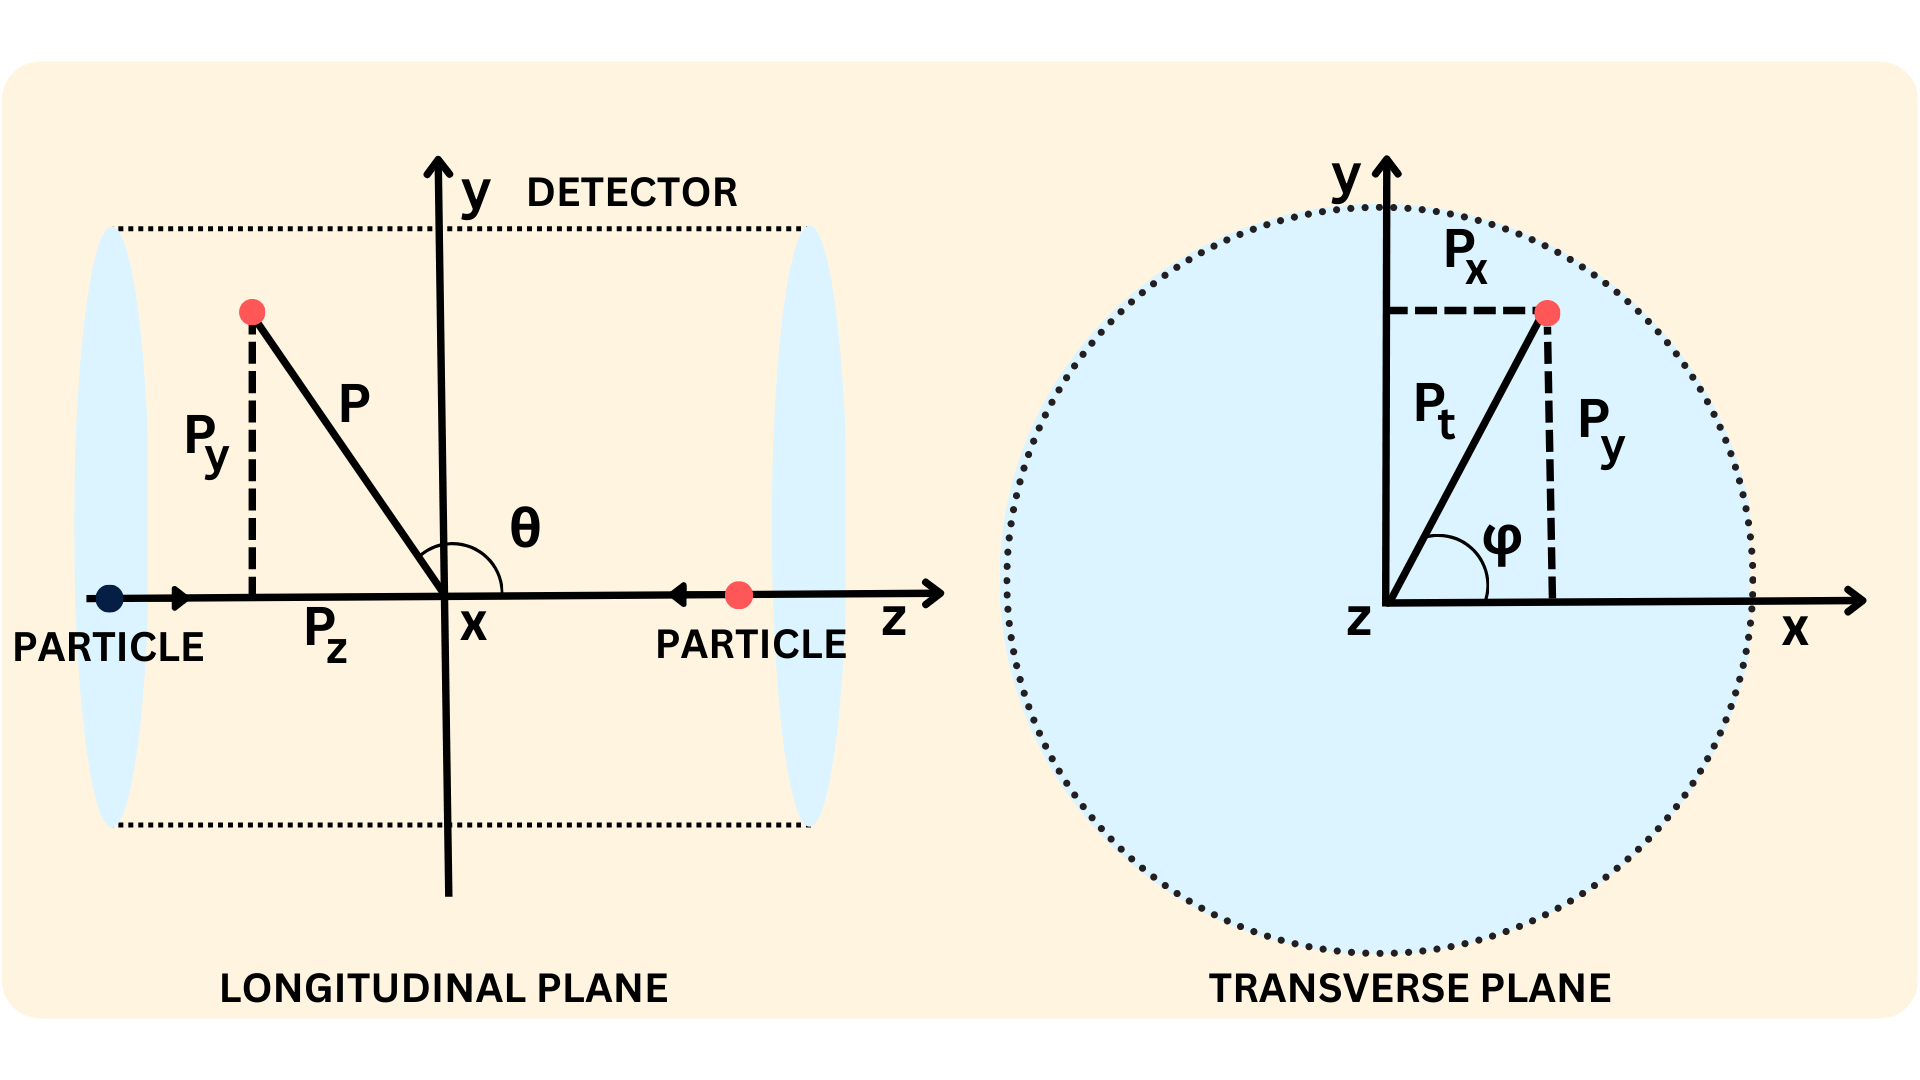
\includegraphics[width=0.65\textwidth]{Figures/Illustrations/Kinematics.png}
    }
    \caption[An illustration of the general kinematics in a particle-collision.]{An illustration of the general kinematics in a particle-collision, 
    inspired by the figure in the thesis by Gramstad \cite{gramstad_searches_nodate}. The illustration shows both the 
    longitudial and transverse plane. }
    \label{fig:Kinematics}
\end{figure}
The transverse momentum and the azimuthal angle are both used in this analysis and are used to create further features. 
Instead of the polar angle, a preferred feature is the pseudorapidity, $\eta$. The pseudorapidity is defined as 
\begin{align}\label{eq:eta}
    \eta = -ln\left[tan\left(\frac{\theta}{2}\right)\right]
\end{align}
The pseudorapidity is preferred to the polar angle because differences in $\eta$ are Lorentz invariant under boosts 
along the longitudinal axis. A large range of features are created using the variables described above. In the appendix I have 
added a summary of all the features used in this analysis (see table \ref{table:Features}). One of these features is the distance 
between the particle in the $\eta\phi-axis$, $\Delta R$. We define $\Delta R$ as 
\begin{align}
    \Delta R = \sqrt{(\Delta \eta)^2 + (\Delta \phi)^2}.
\end{align}
